\documentclass[a4paper,12pt]{article}

% Paquetes básicos
\usepackage[utf8]{inputenc}
\usepackage[T1]{fontenc}
\usepackage[spanish]{babel}
\usepackage{graphicx}
\usepackage{xcolor}
\usepackage{lipsum}
\usepackage{geometry}
\geometry{top=3cm, bottom=3cm, left=2.5cm, right=2.5cm}

% Paquetes para diseño
\usepackage{titlesec}
\usepackage{fancyhdr}
\usepackage{amsmath}
\usepackage{amssymb}
\usepackage{hyperref}

% Paquetes para el entorno lstlisting
\usepackage{listings}
\usepackage{inconsolata}

% Paquete para fondo
\usepackage{background}

% Configuración de lstlisting
\lstset{
    language=Python,
    basicstyle=\ttfamily\small,
    keywordstyle=\color{blue}\bfseries,
    stringstyle=\color{teal},
    commentstyle=\color{gray}\itshape,
    numbers=left,
    numberstyle=\tiny\color{gray},
    backgroundcolor=\color{black!5},
    frame=single,
    rulecolor=\color{black!50},
    breaklines=true,
    captionpos=b,
    showstringspaces=false
}

% Configuración de título
\titleformat{\section}{\normalfont\Large\bfseries}{\thesection}{1em}{}

% Información del documento
\title{
    \vspace{-2cm}
    
\includegraphics[width=0.3\textwidth]{images/fccee.jpg} \\ % Cambia el logo si es necesario
    \LARGE Ingeniería Informática + ADE\\
    \large Universidad de Granada (UGR)\\[1cm]
}
\author{\textbf{Autor:} Ismael Sallami Moreno}
\date{\textbf{Asignatura:} Econometría: Ejercicios Propuestos Solucionados}

% Configuración del fondo
\backgroundsetup{
    scale=1,
    color=black,
    opacity=0.2,
    angle=0,
    position=current page.south,
    vshift=0pt,
    hshift=0pt,
    contents={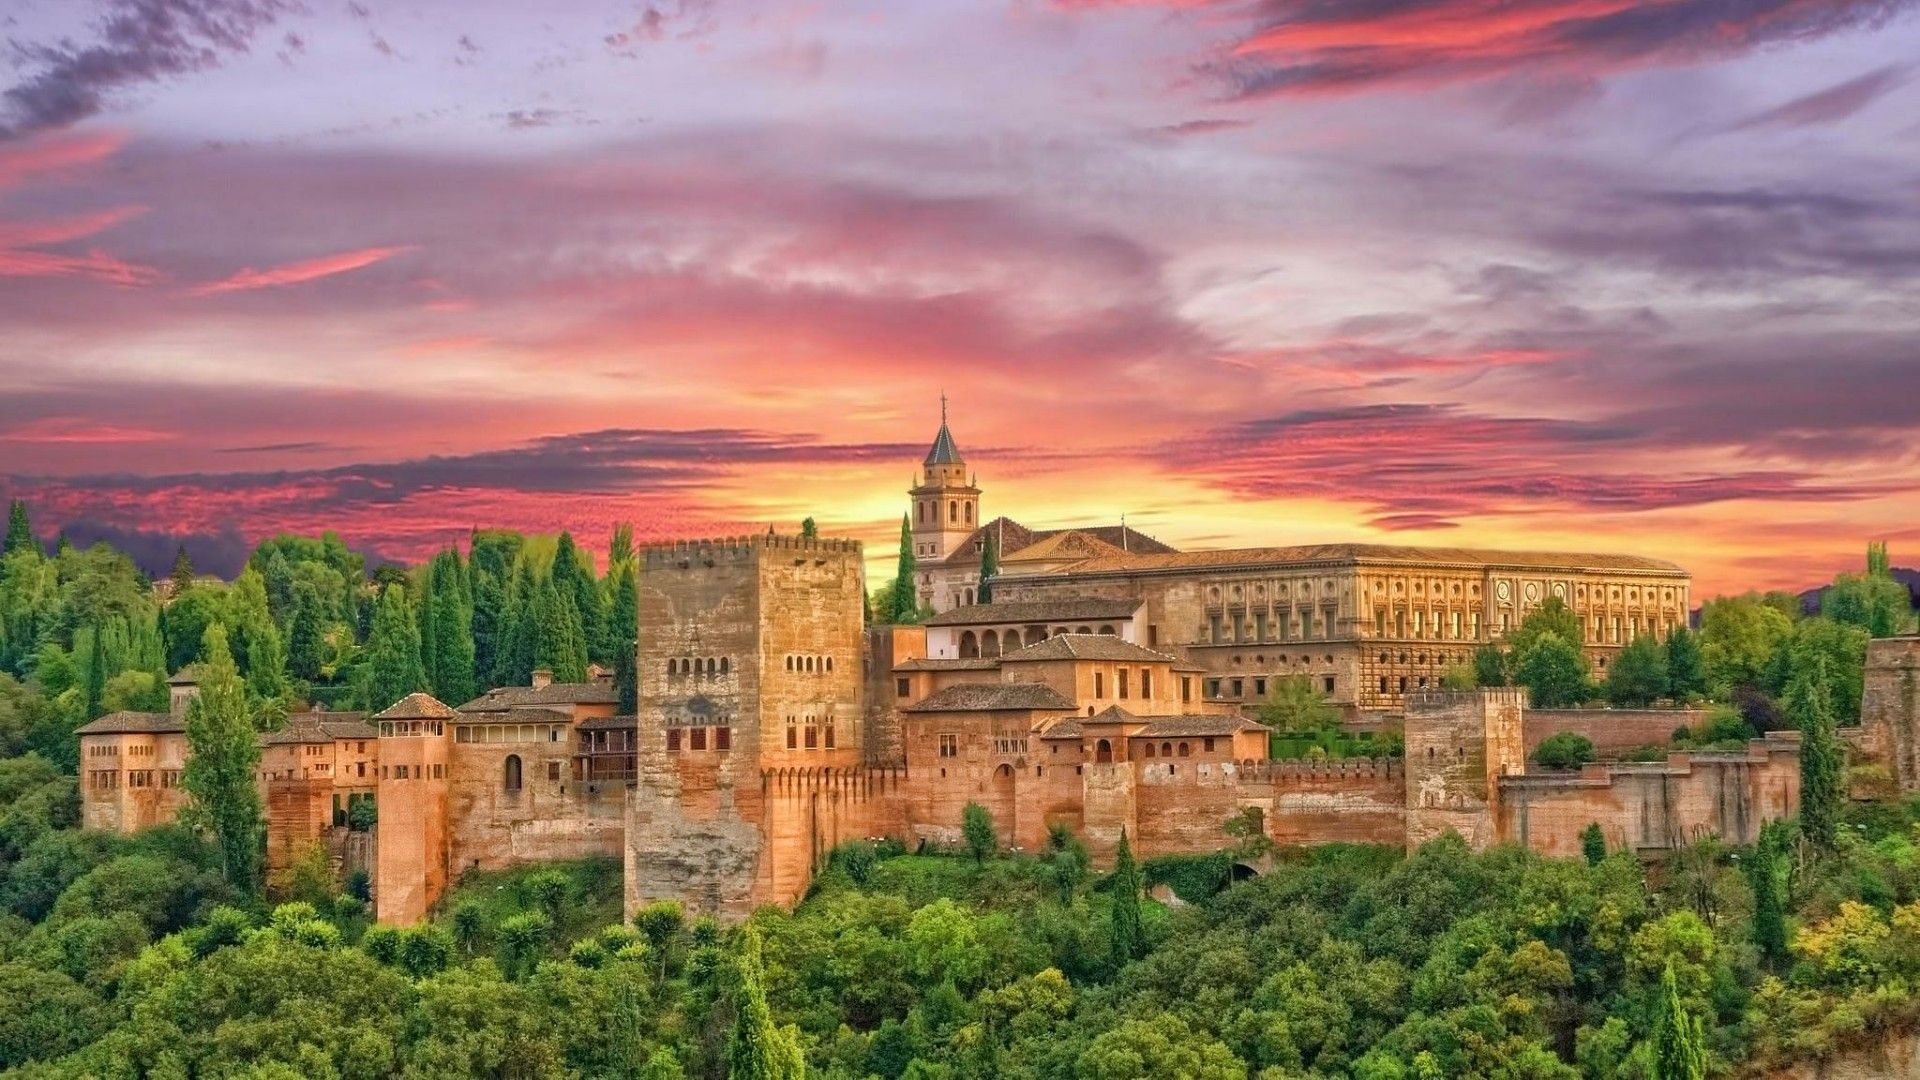
\includegraphics[width=\paperwidth,height=\paperheight,keepaspectratio]{images/granada.jpg}}
}

% Inicio del documento
\begin{document}

% Portada
\maketitle
\thispagestyle{empty}

\begin{center}
    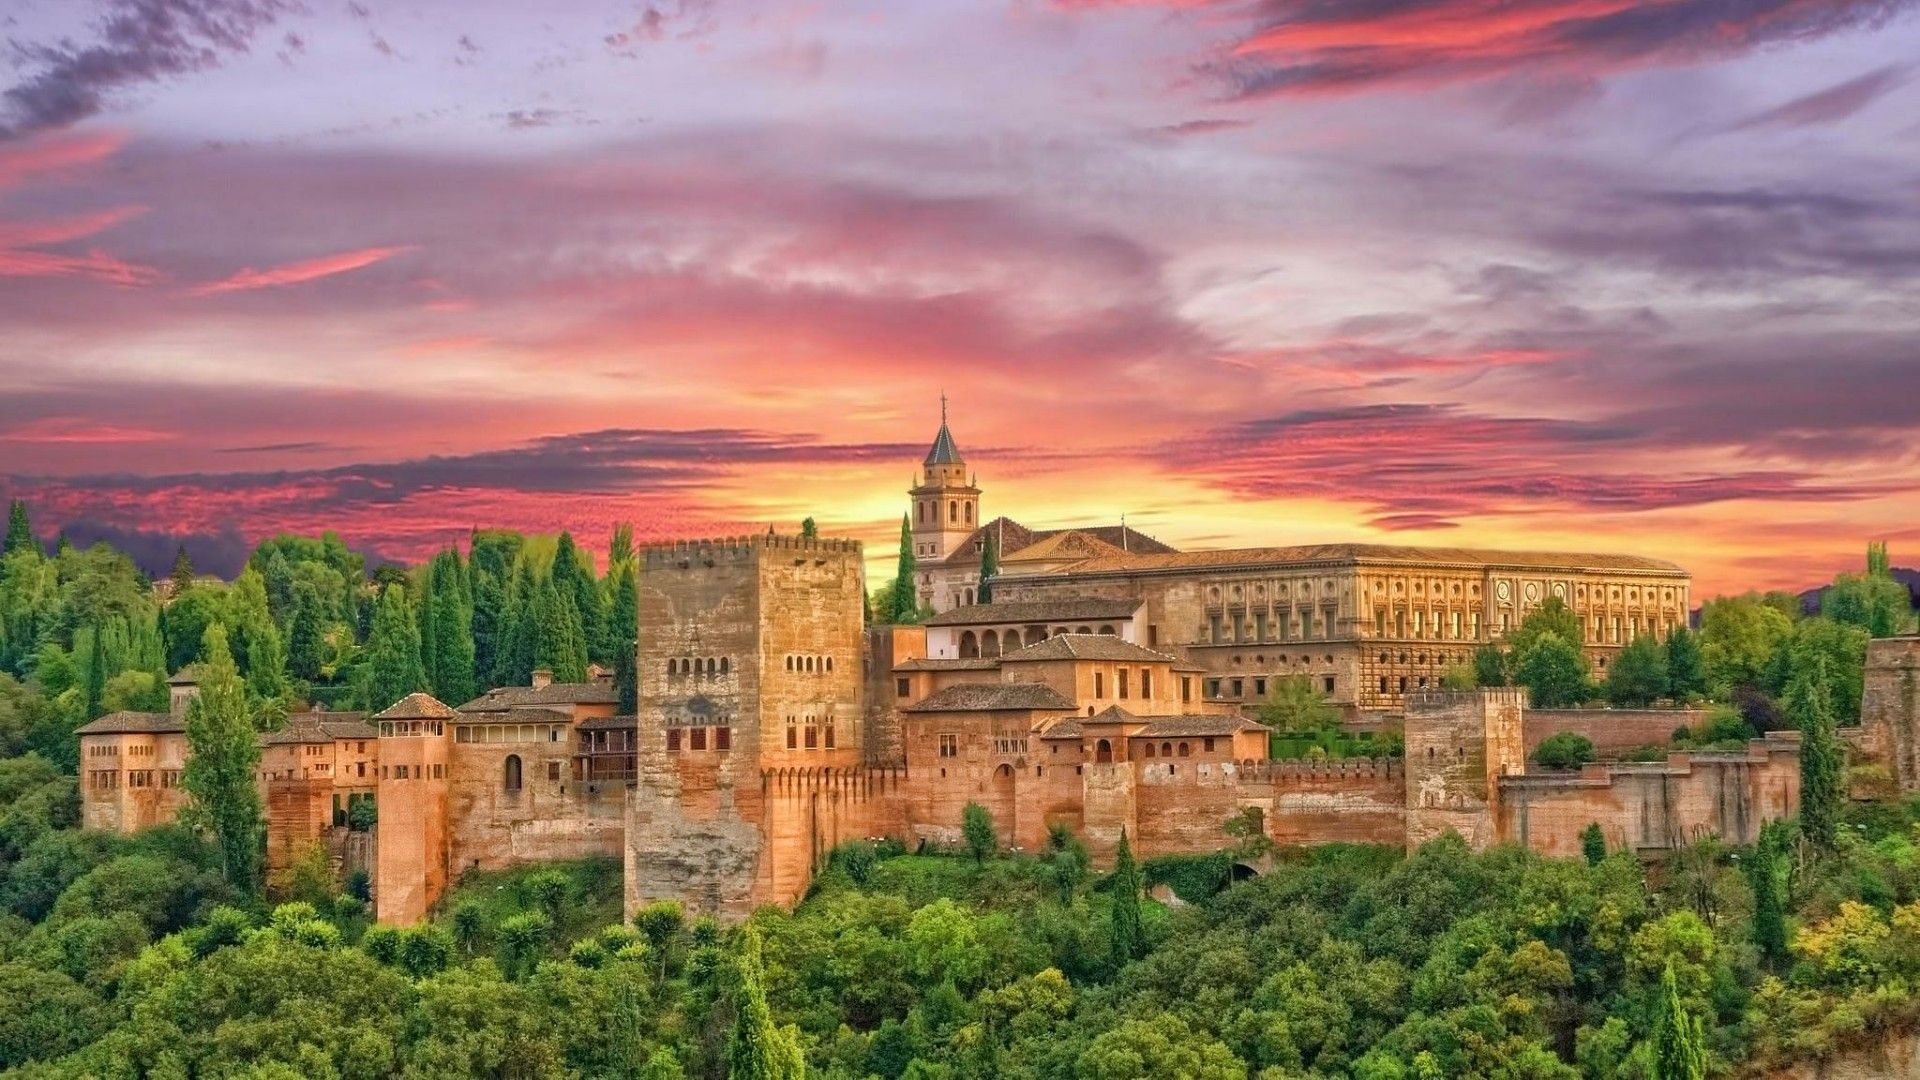
\includegraphics[width=\textwidth,height=0.4\textheight,keepaspectratio]{images/granada.jpg} \\ % Añade tu imagen de fondo
    \vfill
\end{center}

\newpage

% Índice (opcional)
\tableofcontents
\newpage

\section{Tema 2}

\subsection{Ejercicio 1}
\subsection*{Enunciado}
1. Detalle el orden de las matrices y vectores de un modelo econométrico con 3 variables explicativas más el termino constante y 50 observaciones.

\subsection*{Solución}
% El modelo econométrico con 3 variables explicativas más el término constante y 50 observaciones se puede expresar de la siguiente forma:
% \begin{equation}
%     Y = X\beta + \varepsilon
% \end{equation}
% Donde:
% - $Y$ es el vector de resultados (n=50).
% - $X$ es la matriz de variables explicativas (n=50, k=4).
% - $\beta$ es el vector de coeficientes (k=4).
% - $\varepsilon$ es el vector de errores (n=50).
% El orden de las matrices y vectores es:
% - Matriz de variables explicativas $X$ (50x4).
% - Vector de resultados $Y$ (50x1).
% - Vector de coeficientes $\beta$ (4x1).
% - Vector de errores $\varepsilon$ (50x1).

Para ello vamos a suponer que la variable explicada es $Y_t$, si denotamos a las demás varibales explicativas con la simbología $\beta_i$, siendo i el índice de la variable explicativa, podemos nombra a la matriz de variables explicativas como $X$ y a la matriz de coeficientes como $\beta$, y nos queda la siguiente ecuación:  
\begin{equation}
    Y_t = \beta_0 + \beta_1X_{1t} + \beta_2X_{2t} + \beta_3X_{3t} + \beta_4X_{4t} + u_t
\end{equation} 
De manera más sintética, nos quedaría:
\begin{equation}
    \vec{y} = X \vec{\beta} + \vec{u}
\end{equation}

Por lo que podemos decir:
\begin{itemize}
    \item Orden de la matriz $ \vec{y} = (50 x 1)$
    \item Orden de la matriz $ X = (50 x 4)$
    \item Orden de la matriz $ \vec{\beta} = (4 x 1)$
    \item Orden de la matriz $ \vec{u} = (50 x 1)$
\end{itemize}

\subsection{Ejercicio 2}
\subsection*{Enunciado}
2. Ponga un ejemplo de una matriz \( X \) con un término constante y tres variables explicativas de manera que el modelo no cumpla la condición del rango completo por columnas.

\subsection*{Solución}
Una matriz \( X \) con un término constante y tres variables explicativas que no cumpla la condición del rango completo por columnas es aquella en la cual al menos una de las columnas es una combinación lineal de las demás. Por ejemplo:



\[ 
X = \begin{pmatrix}
1 & 2 & 3 & 6 \\
1 & 4 & 5 & 9 \\
1 & 7 & 8 & 15 \\
\end{pmatrix}
\]



En este ejemplo, la cuarta columna es la suma de la segunda y la tercera columnas, lo que significa que el rango de la matriz no es completo.

\subsection{Ejercicio 3}
\subsection*{Enunciado}
3. Razone qué componentes del modelo econométrico tienen carácter estocástico (aleatorio) y cuáles tienen carácter determinista (fijo).

\subsection*{Solución}
En un modelo econométrico típico, hay tanto componentes deterministas como estocásticos.

- \textbf{Componentes deterministas (fijos):}
\begin{itemize}
    \item \textbf{Término constante}: Este es el intercepto del modelo, representado generalmente como \(\beta_0\), y es fijo.
    \item \textbf{Coeficientes de las variables explicativas}: Representados como \(\beta_1, \beta_2, \ldots, \beta_k\), son los parámetros del modelo que permanecen fijos una vez estimados.
\end{itemize}

- \textbf{Componentes estocásticos (aleatorios):}
  \begin{itemize}
    \item \textbf{Término de error}: Representado como \(\epsilon_i\) o \(u_i\), este componente capta la variabilidad no explicada por el modelo y es aleatorio.
  \end{itemize}

Por ejemplo, en el modelo lineal clásico:



\[ 
Y_i = \beta_0 + \beta_1 X_{i1} + \beta_2 X_{i2} + \ldots + \beta_k X_{ik} + \epsilon_i 
\]



Los componentes deterministas son \(\beta_0, \beta_1, \ldots, \beta_k\) y los componentes estocásticos son los \(\epsilon_i\).

\subsection{Ejercicio 4}
\subsection*{Enunciado}
Ponga un ejemplo de una matriz de varianzas-covarianzas de las perturbaciones de un modelo con heterocedasticidad.

\subsection*{Solución}
En un modelo con heterocedasticidad, la varianza de los errores no es constante a lo largo de las observaciones. Un ejemplo de matriz de varianzas-covarianzas de las perturbaciones podría ser:



\[
\Sigma = \begin{pmatrix}
\sigma_1^2 & 0 & 0 \\
0 & \sigma_2^2 & 0 \\
0 & 0 & \sigma_3^2 \\
\end{pmatrix}
\]



donde \(\sigma_1^2\), \(\sigma_2^2\) y \(\sigma_3^2\) son las varianzas de los errores en las diferentes observaciones y son diferentes entre sí, reflejando la presencia de heterocedasticidad.

Por ejemplo:



\[
\Sigma = \begin{pmatrix}
4 & 0 & 0 \\
0 & 9 & 0 \\
0 & 0 & 16 \\
\end{pmatrix}
\]



En este caso, \(\sigma_1^2 = 4\), \(\sigma_2^2 = 9\), y \(\sigma_3^2 = 16\), lo cual indica que las perturbaciones tienen varianzas distintas.

\subsection{Ejercicio 5}
\subsection*{Enunciado}
Ponga un ejemplo de una matriz de varianzas-covarianzas de las perturbaciones de un modelo con autocorrelación.

\subsection*{Solución}
En un modelo con autocorrelación, la matriz de varianzas-covarianzas de las perturbaciones podría tener la siguiente forma:



\[
\Sigma = \begin{pmatrix}
\sigma^2 & \rho \sigma^2 & \rho^2 \sigma^2 \\
\rho \sigma^2 & \sigma^2 & \rho \sigma^2 \\
\rho^2 \sigma^2 & \rho \sigma^2 & \sigma^2 \\
\end{pmatrix}
\]



donde \(\sigma^2\) es la varianza de los errores y \(\rho\) es el coeficiente de autocorrelación. 

Un ejemplo específico podría ser:



\[
\Sigma = \begin{pmatrix}
1 & 0.5 & 0.25 \\
0.5 & 1 & 0.5 \\
0.25 & 0.5 & 1 \\
\end{pmatrix}
\]



En este caso, \(\sigma^2 = 1\) y \(\rho = 0.5\). Esto muestra que las perturbaciones están correlacionadas entre sí, reflejando la presencia de autocorrelación en el modelo.

\subsection{Ejercicio 6}
\subsection*{Enunciado}
6. Se considera la posibilidad de introducir nuevas variables explicativas en el modelo de la curva de Phillips (EJERCICIO 1 de la relación de ejercicios resueltos) y para ello se recoge información sobre la renta nacional disponible neta a precios de mercado por habitante (\(X_2\)) y la renta nacional disponible neta (\(X_3\)).



\[
\begin{array}{|c|c|c|}
\hline
\text{Años} & X_2 & X_3 \\
\hline
2006 & 18614 & 825737 \\
2007 & 19403 & 877724 \\
2008 & 19492 & 896295 \\
2009 & 18719 & 867972 \\
2010 & 18706 & 871015 \\
2011 & 18229 & 851948 \\
2012 & 17822 & 833445 \\
2013 & 17691 & 824821 \\
2014 & 18029 & 837556 \\
2015 & 18828 & 873766 \\
\hline
\end{array}
\]



Se pide:

a) Estimar el modelo incluyendo la variable \(X_2\). (\textbf{Sol.} \(\hat{y} = 165,78 - 1,48X_1 - 0,0077X_2\))

b) Estimar el modelo incluyendo las variables \(X_2\) y \(X_3\). (\textbf{Sol.} \(\hat{y} = 120,97 - 0,77X_1 - 0,017X_2 + 0,00025X_3\))

c) Comparar ambos modelos. (\textbf{Sol.} \(R^2_1 = 0,7097 < R^2_2 = 0,96; AIC_1 = 2,83 > AIC_2 = 0,8920\))

\subsection*{Solución}
\begin{itemize}
  \item \textbf{Modelo incluyendo la variable \(X_2\)}:
  

\[
  \hat{y} = 165,78 - 1,48X_1 - 0,0077X_2
  \]



  Para estimar este modelo, hemos utilizado una regresión lineal múltiple donde \(X_1\) es la variable original del modelo de la curva de Phillips y \(X_2\) es la nueva variable explicativa añadida (renta nacional disponible neta a precios de mercado por habitante). Los coeficientes \(165,78\) (intercepto), \(-1,48\) (coeficiente de \(X_1\)), y \(-0,0077\) (coeficiente de \(X_2\)) han sido estimados a partir de los datos proporcionados usando el método de mínimos cuadrados ordinarios (MCO).

  \textbf{Para ello:}

  \begin{itemize}
    \item Debemos de calcular los siguiente valores:
    \begin{align*}
        \sum_{i=1}^{10} X_{1_i} & \\
        \sum_{i=1}^{10} X_{1_i}^2 & \\
        \sum_{i=1}^{10} X_{2_i} & \\
        \sum_{i=1}^{10} X_{2_i}^2 & \\
        \sum_{i=1}^{10} X_{1_i}Y_{t} & \\
        \sum_{i=1}^{10} X_{2_i}Y_{t} & \\
        \sum_{i=1}^{10} Y_{t} &
    \end{align*}
    \item Con estos valores calculamos la siguiente matriz:
    \begin{equation*}
        X^{\prime}X = \begin{pmatrix}
            n & \sum_{i=1}^{10} X_{1_i} & \sum_{i=1}^{10} X_{2_i} \\
            \sum_{i=1}^{10} X_{1_i} & \sum_{i=1}^{10} X_{1_i}^2 & \sum_{i=1}^{10} X_{1_i}X_{2_i} \\
            \sum_{i=1}^{10} X_{2_i} & \sum_{i=1}^{10} X_{1_i}X_{2_i} & \sum_{i=1}^{10} X_{2_i}^2
        \end{pmatrix}
    \end{equation*}

    \item Y calculamos de manera análoga la siguiente matriz:
    \begin{equation*}
        X^{\prime}Y = \begin{pmatrix}
            \sum_{i=1}^{10} Y_{t} \\
            \sum_{i=1}^{10} X_{1_i}Y_{t} \\
            \sum_{i=1}^{10} X_{2_i}Y_{t}
        \end{pmatrix}
    \end{equation*}

    \item Por último, calculamos la matriz del estimador, aplicando el estimador de MCO:
    \begin{equation*}
        \hat{\beta} = (X^{\prime}X)^{-1}X^{\prime}Y
    \end{equation*}

    % Para ver el apartado a), pinche \href{https://github.com/ElblogdeIsmael/ElblogdeIsmael.github.io/tree/main/Asignaturas/Tercer%20A%C3%B1o/ECO/Practicas/EjerciciosPropuestos/SolucionesEjercicios/Tema2}{aquí} y visualice el archivo en formato .xlsx

  \end{itemize}

  \item \textbf{Modelo incluyendo las variables \(X_2\) y \(X_3\)}:
  

\[
  \hat{y} = 120,97 - 0,77X_1 - 0,017X_2 + 0,00025X_3
  \]



  De manera similar, para este modelo se ha llevado a cabo una regresión lineal múltiple incluyendo ahora tanto \(X_2\) como \(X_3\) (renta nacional disponible neta total). Los coeficientes \(120,97\) (intercepto), \(-0,77\) (coeficiente de \(X_1\)), \(-0,017\) (coeficiente de \(X_2\)), y \(0,00025\) (coeficiente de \(X_3\)) han sido obtenidos mediante el método de MCO.

  \item \textbf{Comparación de ambos modelos}:
  \begin{itemize}
    \item Coeficiente de determinación ajustado (\(R^2\)):
    

\[
    R^2_1 = 0,7097 \quad \text{(modelo con \(X_2\) solamente)} < R^2_2 = 0,96 \quad \text{(modelo con \(X_2\) y \(X_3\))}
    \]


    El coeficiente de determinación ajustado (\(R^2\)) indica el porcentaje de variabilidad en la variable dependiente que es explicado por las variables independientes. En este caso, el modelo que incluye \(X_2\) y \(X_3\) explica el \(96\%\) de la variabilidad en \(Y\), mientras que el modelo con sólo \(X_2\) explica el \(70,97\%\).

    \item Criterio de Información de Akaike (AIC):
    

\[
    AIC_1 = 2,83 \quad \text{(modelo con \(X_2\) solamente)} > AIC_2 = 0,8920 \quad \text{(modelo con \(X_2\) y \(X_3\))}
    \]


    El AIC es una medida de la calidad del modelo relativo a otros modelos. Un menor AIC indica un mejor ajuste del modelo. En este caso, el modelo con \(X_2\) y \(X_3\) tiene un AIC menor (0,8920) comparado con el modelo que incluye sólo \(X_2\) (2,83), indicando que el modelo con ambas variables explicativas \(X_2\) y \(X_3\) es superior en términos de ajuste.
  \end{itemize}
\end{itemize}

Para realizar el apartado c), hemos usado estan funciones:

     \begin{equation}
        R^2 = \frac{\frac{1}{n} \cdot \sum_{i=1}^{n} \left( \hat{Y}_i - \bar{Y} \right)^2}{\frac{1}{n} \cdot \sum_{i=1}^{n} \left( Y_i - \bar{Y} \right)^2} = \frac{\sum_{i=1}^{n} \left( \hat{Y}_i - \bar{Y} \right)^2}{\sum_{i=1}^{n} \left( Y_i - \bar{Y} \right)^2} = \frac{SCE}{SCT}
        \end{equation}
     \begin{equation}
        SCE = \hat{\beta}^{T} \cdot X^{\prime}Y - 10 \cdot \left(\frac{\sum_{i=1}^{10}Y}{n}\right)^{2}    
    \end{equation}

    
    
Y para el cálculo de AIC:
\begin{equation}
    AIC = ln (\frac{SCR}{n}) \cdot \frac{2k}{n}
\end{equation}
Siendo k el número de variables explicativas y n el número de observaciones.
Para encontrar los calculos pincha \href{https://github.com/ElblogdeIsmael/ElblogdeIsmael.github.io/tree/main/Asignaturas/Tercer%20A%C3%B1o/ECO/Practicas/EjerciciosPropuestos/SolucionesEjercicios/Tema2}{aquí} y visualiza el archivo en formato .xlsx

\subsection{Ejercicio 7}
\subsection*{Enunciado}

En la siguiente tabla se recogen las ventas de seis empresas informáticas en función del número de comerciales:

\[
\begin{array}{c|cccccc}
v_t & 109 & 111 & 132 & 140 & 169 & 180 \\
\hline
c_t & 12 & 15 & 17 & 18 & 19 & 20 \\
\end{array}
\]



Se pide:

\begin{enumerate}
    \item[a)] Plantear el modelo econométrico y estimar los coeficientes por mínimos cuadrados ordinarios. Interpretación de los coeficientes estimados. (Sol. $\hat{v}_t = -13,56 + 9,132c_t$)
    \item[b)] Calcular el coeficiente de determinación e interpretarlo. ($R^2 = 0,8294$)
    \item[c)] Se estima un modelo alternativo añadiendo como variable explicativa el gasto en publicidad de cada empresa, obteniendo un coeficiente de determinación igual a 0,93363. Concluya de forma razonada si este modelo es mejor que el anterior. (Sol. $\bar{R}^2_1 = 0,78675 < \bar{R}^2_2 = 0,8893$)
\end{enumerate}

\subsection*{Solución}

Para ello debemos de realizar los mismo pasos que en el ejercicio anterior para la resolución del apartado a y b, y para el c basta con calcular el coeficiente de determinación ajustado y compararlos (Usando las fórmulas expuestas anteriormente).

\subsection{Ejercicio 8}

\subsection*{Enunciado}
Se tiene la siguiente información correspondiente al curso 2010/2011 sobre el número de becarios en la enseñanza universitaria (\(Y\)), el alumnado matriculado en estudios de 1er. y 2º ciclo y de grado (\(X_1\)) y el importe en miles de euros de las becas (\(X_2\)). Se pide:

\begin{table}[h!]
\centering
\begin{tabular}{|l|r|r|r|}
\hline
CCAA & \(Y\) & \(X_1\) & \(X_2\) \\
\hline
Andalucía & 97.105 & 234.851 & 266.222,60 \\
Aragón & 9.294 & 31.063 & 19.648,80 \\
Asturias & 6.882 & 23.746 & 16.048,00 \\
Baleares & 4.251 & 15.488 & 8.224,60 \\
Canarias & 19.125 & 41.546 & 45.084,30 \\
Cantabria & 4.078 & 8.157 & 5.011,80 \\
Castilla y León & 27.307 & 78.694 & 75.124,10 \\
Castilla - La Mancha & 8.380 & 30.856 & 20.717,00 \\
Cataluña & 51.965 & 179.637 & 138.077,10 \\
Valencia & 49.805 & 148.671 & 115.219,30 \\
Extremadura & 12.088 & 22.747 & 35.506,00 \\
Galicia & 24.500 & 64.262 & 66.019,40 \\
Madrid & 64.563 & 239.389 & 134.341,50 \\
Murcia & 15.549 & 42.573 & 37.177,90 \\
Navarra & 4.669 & 14.705 & 10.372,50 \\
País Vasco & 15.322 & 53.419 & 26.789,40 \\
Rioja, La & 1.761 & 8.119 & 3.345,10 \\
A distancia & 20.557 & 212.021 & 16.491,60 \\
\hline
\end{tabular}
\end{table}

a) Estimar los parámetros. (Sol. \(\hat{y} = 528,077 + 0,09X_1 + 0,2936X_2\))

b) Obtener el coeficiente de determinación. (Sol. \(R^2 = 0,994\))

c) Obtener el coeficiente de determinación corregido. (Sol. \(\bar{R}^2 = 0,993\))

d) Calcular el criterio de Akaike. (Sol. \(AIC = 328,9392\))

\subsection*{Solucion}
Similar a los ejercicios anteriores en cuanto al cálculo de AIC y BIC basta con aplicar las fórmulas expuestas en la teoría.

\begin{equation}
    AIC = ln (\frac{SCR}{n}) + \frac{2k}{n}
\end{equation}

\begin{equation}
    BIC = ln (\frac{SCR}{n}) + \frac{k}{n} \cdot ln(n)
\end{equation}

\subsection{Resto de ejercicios}
Para la resolución del resto de ejercicios basta con seguir la misma lógica que en los ejercicios anteriores, aplicando las fórmulas expuestas en la teoría. Puede servirse de la hoja de cálculo que se ha proporcionado en el apartado anterior para realizar los cálculos de manera más sencilla.


\section{Tema 3}




\end{document}
